\subsection{MUSIC-algoritmi}
\cite{Schmidt1986MultipleEstimation} kehitti usean signaalin luokittelu -algoritmin (Multiple Signal Classification, MUSIC), joka perustuu mittausdatan jakamiseen keskenään ortogonaalisiin signaali- ja kohina-aliavaruuksiin, jonka jälkeen tarkistetaan potentiaalisen lähdepisteen topografian kuuluminen signaaliavaruuteen \citep{Mosher1999SourceMUSIC}. Algoritmissa lähteet kuvataan sähköisinä dipoleina ja algoritmi vaatii päämalliin tehdyn suoran mallin (forward model).

Dipolit aivoissa voidaan olettaa kiinnitetyiksi eli niiden sijainnit eivät muutu ajan suhteen. MUSIC-algoritmit voidaan jakaa kahteen kategoriaan riippuen, miten dipolien suuntautumiset oletetaan olevan. Dipolit voivat olla joko kiinteästi suuntautuneita eli niiden suuntautuminen tiedetään etukäteen tai vapaasti suuntautuvia, jolloin niiden suuntausta ei tiedetä. \citep{Makela2018TruncatedLocalization}

-Tähän pitäisi kirjoittaa MUSICin peruskäsitteet

Aloitetaan esittelemällä kiinnitetyn orientaation MUSIC-algoritmi, jota kutsutaan myös nimellä skalaari-MUSIC \citep{Makela2018TruncatedLocalization}. 

Olkoon pisteessä $\mathbf{p}$ dipoli, jolla on orientaatio $\eta$. Yhden sensorin lukema data on muotoa $\mathbf{y(t) = As(t)+\epsilon(t)}$, jossa \textbf{A} on sekoitusmatriisi, 

Olkoon mittauksista saatu data-matriisi $\mathbf{Y}\in \mathbb{R}^{m\times N}$, jossa $\mathit{m}$ on mittaussensorien määrä ja $\mathit{N}$ mittausten lukumäärä. Matriisilla $\mathbf{Y}$ on muoto

\begin{equation}
    \mathbf{Y=AS+\epsilon},
\end{equation}
jossa $\mathbf{A =[l(p}_1,\eta_1),...,\mathbf{l(p}_n,\eta_n)]$ on sekoitusmatriisi, $\mathbf{S}$ ajankulkumatriisi ja $\mathbf{\epsilon}$ mittauskohinaa. Lähteen orientaatio on kiinnitetyn orientaation tapauksessa riippuvainen vain sen sijainnista eli $\mathbf{l(p},\eta)=\mathbf{L(p})\mathbf{\eta}(\mathbf{p})$, jossa $\mathbf{L(p) = [l(p,e_x),l(p,e_y),l(p,e_z)]}$ on johtokenttämatriisi (lead field matrix).

Data-avaruus $\text{span}(\mathbf{Y})$ jaetaan singulaariarvohajotelman avulla kahteen keskenään ortogonaaliseen aliavaruuteen, signaali-avaruuteen $\text{span}(\mathbf{A})$  ja kohina-avaruuteen $\text{span}(\mathbf{A^\bot})$ \citep{Mosher1999SourceMUSIC}. Olkoon matriisin \textbf{Y} singulaariarvohajotelma muotoa $\mathbf{Y = UDV}^T$ ja lähteiden määrä \textit{n}. Matriisin \textbf{D} diagonaalilla olevat \textit{n} ensimmäistä ominaisarvoa kuvaavat signaalia ja loput ominaisarvot kohinaa. Tällöin matriisin sarakkeet $\mathbf{U}(:,1:n)$ virittävät signaaliavaruuden eli $\text{span}(\mathbf{A}) = \mathbf{U}(:,1:n)$. \citep{Mosher1999SourceMUSIC, Makela2018TruncatedLocalization}

Ortogonaaliprojektio signaaliavaruuteen $\text{span}(\mathbf{A})$ voidaan approksimoida kaavan (\ref{eq:6}) avulla

\begin{equation}
    \mathbf{P}_{sg}=\mathbf{U}(:,1:n)\mathbf{U}(:,1:n)^T
\end{equation} \citep{Makela2018TruncatedLocalization}

Lähteiden määrää ei aina tiedetä, joten se täytyy approksimoida. Datamatriisin ominaisarvoista voidaan päätellä, kuinka monta voimakasta lähdettä löydetään signaaliavaruudesta. Ominaisarvoista voidaan muodostaa pylväsdiagrammi ja lähteiden määrä voidaan approksimoida sen mukaan, missä kohdassa tapahtuu merkittävä pudotus. Valkoisen kohinan tapauksessa pylväät tasoittuvat loppupäässä, kun lähteet ovat loppuneet. Värillisellä kohinalla pudotuksen löytäminen on hankalampaa ja täten lähteiden approksimaatio on vaikeampaa. Kuvassa \ref{fig:D} on simuloidun mittausdatan ominaisarvot pylväsdiagrammeina valkoisen ja värillisen kohinan tapauksissa.

Olkoon approksimoitujen lähteiden määrä \~{n}. Projektio voidaan nyt muodostaa approksimoitujen lähteiden määrän mukaan $\mathbf{P}_{s}=\mathbf{U}(:,1:\~n)\mathbf{U}(:,1:\~n)^T$, jolloin \~n jälkeiset ominaisvektorit kuvaavat kohinaa.

\begin{figure}[h]
    \centering
    \begin{minipage}{0.5\textwidth}
        \centering
        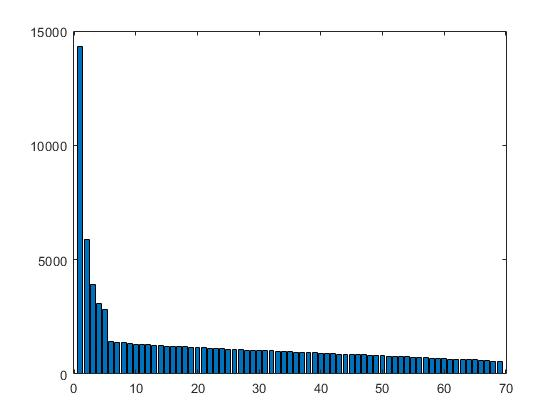
\includegraphics[width=1\textwidth]{d_valk.jpg} 
    \end{minipage}
    \begin{minipage}{0.5\textwidth}
        \centering
        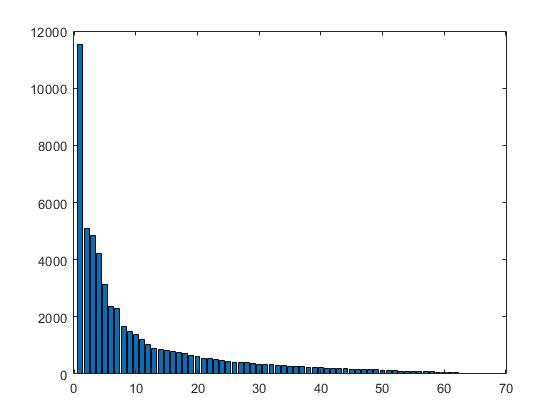
\includegraphics[width=1\textwidth]{d_var.jpg}
    \end{minipage}
    \caption{Vasemman puoleisessa kuvassa simuloitu data sisältää valkoista kohinaa ja oikean puoleisessa kuvassa värillistä kohinaa. Molemmissa simulaatioissa on viisi lähdettä ja kohinan määrä on yhtä suuri.}
    \label{fig:D}
\end{figure}

Pisteen $\mathbf{p}$ kuuluminen signaaliavaruuteen tarkistetaan projektio-operaattorin avulla. Pisteen $\mathbf{p}$ topografia $\mathbf{l(p)}$ lasketaan päämallin avulla. Topografia kuuluu signaaliavaruuteen, jos sen projektio signaaliavaruuteen on topografia itse. Toisin sanoen piste $\mathbf{p}$ on lähde, jos $\mathbf{P}_s\mathbf{l(p)} = \mathbf{l(p)}$. Tämä tarkoittaa sitä, että jos $\mathbf{l(p)}$ sijaitsee signaaliavaruudessa, sen normi ei muutu projektiossa eli $||\mathbf{P}_s\mathbf{l(p)}||=||\mathbf{l(p)}||$. Jos $\mathbf{l(p)}$ ei sijaitse signaaliavaruudessa, sen projektion normi on pienempi kuin $\mathbf{l(p)}$:n normi eli
$||\mathbf{P}_s\mathbf{l(p)}||<||\mathbf{l(p)}||$. \citep{Makela2018TruncatedLocalization}

Näistä saadaan muodostettua paikannusfunktio (localizer function) \citep{Makela2018TruncatedLocalization}, joka laskee jokaisen pisteen $\mathbf{p}$ kuulumisen signaaliavaruuteen

\begin{equation}
    \mathbf{\mu(p)} = \frac{||\mathbf{P}_s\mathbf{l(p)}||^2}{||\mathbf{l(p)}||^2} 
    \begin{cases}
    =1\text{, jos p on lähde}\\
    <1\text{, jos p ei ole lähde}
     \end{cases}
\end{equation}

Vapaan orientaation tapauksessa jokaiselle pisteelle $\mathbf{p}$ määräytyy suuntaus $\mathbf{\eta}$ mittausdatan perusteella. Vapaan orientaation MUSIC-algoritmia kutsutaan myös nimellä vektori-MUSIC \citep{Makela2018TruncatedLocalization}. Vektori-MUSIC muodostetaan hyvin samalla tavalla kuin skalaari-MUSIC, mutta sen paikannusfunktio on erilainen

\begin{equation}
    \mathbf{\mu(p)} = \max_{||\eta||=1} \frac{||\mathbf{P}_s\mathbf{L(p)\eta}||^2}{||\mathbf{L(p)\eta}||^2}
\end{equation}

(jatkuu kunhan opin selittämään)